\let\negmedspace\undefined
\let\negthickspace\undefined
\documentclass[journal]{IEEEtran}
\usepackage[a5paper, margin=10mm, onecolumn]{geometry}
\usepackage{tfrupee} 
\setlength{\headheight}{1cm} 
\setlength{\headsep}{0mm}     

\usepackage{gvv-book}
\usepackage{gvv}
\usepackage{cite}
\usepackage{amsmath,amssymb,amsfonts,amsthm}
\usepackage{algorithmic}
\usepackage{graphicx}
\usepackage{textcomp}
\usepackage{xcolor}
\usepackage{txfonts}
\usepackage{listings}
\usepackage{enumitem}
\usepackage{mathtools}
\usepackage{gensymb}
%\usepackage{wasysym}
\usepackage{comment}
\usepackage[breaklinks=true]{hyperref}
\usepackage{tkz-euclide} 
\usepackage{listings}
\def\inputGnumericTable{}                                 
\usepackage[latin1]{inputenc}                                
\usepackage{color}                                            
\usepackage{array}                                            
\usepackage{longtable}                                       
\usepackage{calc}                                             
\usepackage{multirow}                                         
\usepackage{hhline}                                           
\usepackage{ifthen}                                           
\usepackage{lscape}
\usepackage{circuitikz}
\tikzstyle{block} = [rectangle, draw, fill=blue!20, 
    text width=4em, text centered, rounded corners, minimum height=3em]
\tikzstyle{sum} = [draw, fill=blue!10, circle, minimum size=1cm, node distance=1.5cm]
\tikzstyle{input} = [coordinate]
\tikzstyle{output} = [coordinate]
\renewcommand{\thefigure}{\theenumi}
\renewcommand{\thetable}{\theenumi}
\setlength{\intextsep}{10pt} % Space between text and floats
\numberwithin{equation}{enumi}
\numberwithin{figure}{enumi}
\renewcommand{\thetable}{\theenumi}

\begin{document}

\bibliographystyle{IEEEtran}
\vspace{3cm}

\title{5.8.30}
\author{EE25BTECH11032 - Kartik Lahoti}
\maketitle

\subsection*{Question: } 
Rambha travels $300\,km$ to her home partly by train and partly by bus. She takes $4$ hours 
if she travels $60\,km$ by train and the remaining by bus. If she travels $100\,km$ by train and the remaining by bus, she takes $10$ minutes longer. Find the speed of the train and the bus seperately.\\

\textbf{Solution}:\\

Given, 
\begin{table}[H]
    \centering
    \begin{tabular}{|c|c|}
\hline
\textbf{Name} & \textbf{Value} \\
\hline
Circle & $\vec{x}^\top\vec{x} - a^2 = 0$ \\
\hline
Line & $\vec{x} = \myvec{\tfrac{a}{\sqrt{2}} \\ 0} + \kappa\myvec{0 \\ 1}$ \\
\hline
\end{tabular}

    \caption*{5.8.30}
    \label{table_1}
\end{table}

Let the equations be,

\begin{align}
    \vec{n_1}^{\top}\vec{X} = c_1 \\ 
    \vec{n_2}^{\top}\vec{X} = c_2 
\end{align}

Since $\vec{P}$ satisfies both the lines, 

\begin{align}
    \vec{n_1}^{\top}\vec{P} = c_1 \\ 
    \vec{n_2}^{\top}\vec{P} = c_2 
\end{align}

Solving for $\vec{P}$

\begin{align}
    \augvec{2}{1}{60 & 240 & 4\\100 & 200 & \frac{25}{6}}\xleftrightarrow[]{R_1\rightarrow \frac{R_1}{60}}\augvec{2}{1}{1 & 4 & \frac{1}{15}\\100 & 200 & \frac{25}{6}}
\end{align}
\begin{align}
    \augvec{2}{1}{1 & 4 & \frac{1}{15}\\100 & 200 & \frac{25}{6}}\xleftrightarrow[]{R_2\rightarrow \frac{R_2}{100}}\augvec{2}{1}{1 & 4 & \frac{1}{15}\\1 & 2 & \frac{1}{24}}
\end{align}

\begin{align}
    \augvec{2}{1}{1 & 4 & \frac{1}{15}\\1 & 2 & \frac{1}{24}}\xleftrightarrow[]{R_2\rightarrow R_2 - R_1}\augvec{2}{1}{1 & 4 & \frac{1}{15}\\0 & -2 & \frac{-1}{40}}
\end{align}

\begin{align}
    \augvec{2}{1}{1 & 4 & \frac{1}{15}\\0 & -2 & \frac{-1}{40}} \xleftrightarrow[]{R_2\rightarrow \frac{R_2}{-2} }\augvec{2}{1}{1 & 4 & \frac{1}{15}\\0 & 1 & \frac{1}{80}}
\end{align}

\begin{align}
    \augvec{2}{1}{1 & 4 & \frac{1}{15}\\0 & 1 & \frac{1}{80}} \xleftrightarrow[]{R_1\rightarrow R_1 - 4R_2 }\augvec{2}{1}{1 & 0 & \frac{1}{60}\\0 & 1 & \frac{1}{80}}
\end{align}

\begin{align}
    \therefore \vec{P} = \myvec{\frac{1}{60} \\ \frac{1}{80}}
\end{align}

Since $\vec{P}$ is the reciprocal of the speeds 

The speed of train is $60\,km/h$ and bus is $80\,km/h$

\begin{figure}[H]
    \centering
    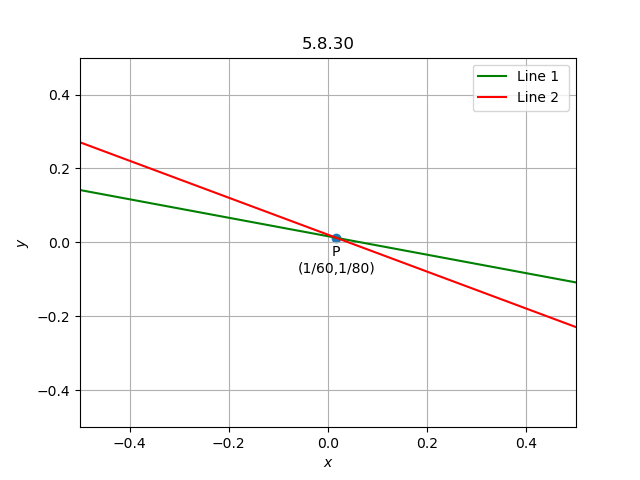
\includegraphics[width=1.0\columnwidth]{figs/Inter1.png}
    \caption*{}
    \label{fig:placeholder}
\end{figure}

\end{document}


